\documentclass{article}
\usepackage{abstract}
\usepackage{url}
\usepackage[top=2cm, bottom=2cm, left=2.3cm, right=2.3cm]{geometry}
\renewcommand{\abstractnamefont}{\Large}
\renewcommand{\abstracttextfont}{\normalfont}
\usepackage[utf8]{inputenc}
\usepackage{graphicx}
\usepackage{booktabs}
\usepackage{tikz}
\usepackage{float}
\usepackage{indentfirst}
\oddsidemargin 0pt
\evensidemargin 0pt
\marginparwidth 40pt
\marginparsep 10pt
\topmargin -20pt
\headsep 10pt
\textheight 8.7in
\textwidth 6.65in
\linespread{1.4}

\nocite{*}
\usepackage{biblatex} %Imports biblatex package
\addbibresource{reference.bib} %Import the bibliography file

%% Title
\title{
		\usefont{OT1}{bch}{b}{n}
		BIS634 Final Project \\
		COVID-19 Vaccine Tweets Analysis\\
}

\author{Shurui Wang (sw2349)}
\date{December 15, 2022}


\begin{document}
\maketitle
\thispagestyle{empty}
\newpage
\pagenumbering{arabic} 
\section{Introduction}

This research is mainly based on the COVID-19 vaccine tweets dataset. After cleaning and integrating the data, I used Plotly to visualize the data and created several interactive plots. To better present the results, I have created a local Web application with Python Flask that contains everything I have obtained from this research.

\section{Data}

In this research, I used a Kaggle dataset named COVID-19 vaccine tweets. This dataset contains tweets about the COVID-19 vaccines used in the entire world, with the following vaccines:
\begin{itemize}
  \item Pfizer/BioNTech
  \item Sinopharm
  \item Sinovac
  \item Moderna
  \item Oxford/AstraZeneca
  \item Covaxin
  \item Sputnik V
\end{itemize}

\subsection{Basic Information}

\subsubsection{Data Description}

The original dataset has 228207 rows and 16 columns. Each row represents a tweet, with user information, date(from 2020-12-12 to 2021-11-23), and the tweet's attributes recorded in different columns. In this project, I only need three columns out of 16 columns, which are text, user\_location, and date.

text: The complete text of a tweet. Hashtags, emojis and symbols are included.

date: The exact date and time of the tweet.

user\_location: The location user selected when tweeting, which is not necessarily the user's actual location.

Here is an overview of the dataset:

\begin{figure}[H]
\centering
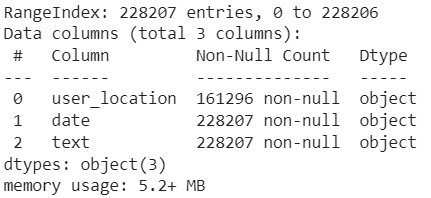
\includegraphics[width=8cm]{df2.png}
\caption{Dataset Information}
\end{figure}

\begin{figure}[H]
\centering
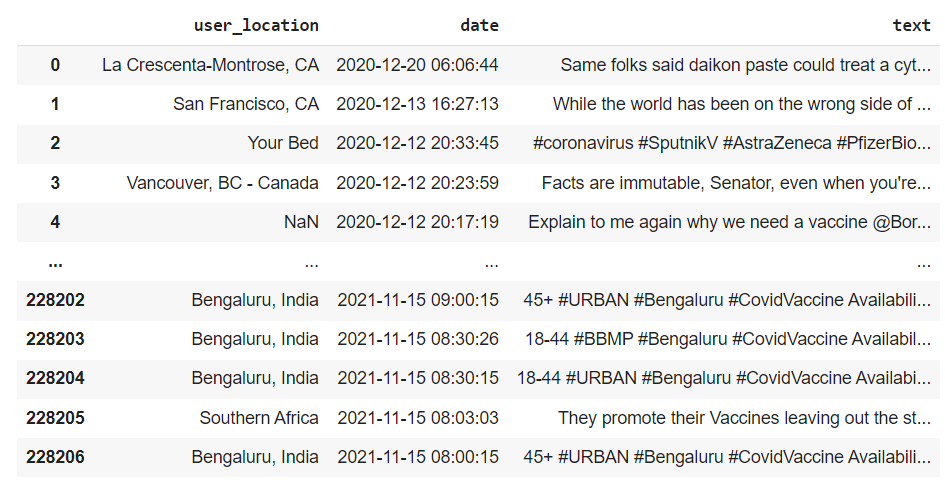
\includegraphics[width=15cm]{df.png}
\caption{Vaccine Tweets Dataset Overview}
\end{figure}

Noticed that there are missing values in the user\_location column. This is because not all users will include their locations while tweeting. Since the text and date columns don't have missing values, I will leave the user\_location column untouched.

\subsubsection{Why is it interesting?}
The COVID-19 pandemic keeps affecting our lives in the past few years. Vaccinations are essential to protect ourselves from COVID, however, some people may hesitate of taking the vaccine, while others may suffer from adverse effects after taking the vaccine. As shown in the below figure, the vaccination rate gets higher and higher in 2021, how people think about vaccines and their feedback after taking the vaccines are worth looking at. It is also interesting to analyze the variations in the sentiment with respect to time, vaccine, and country.

\begin{figure}[H]
\centering
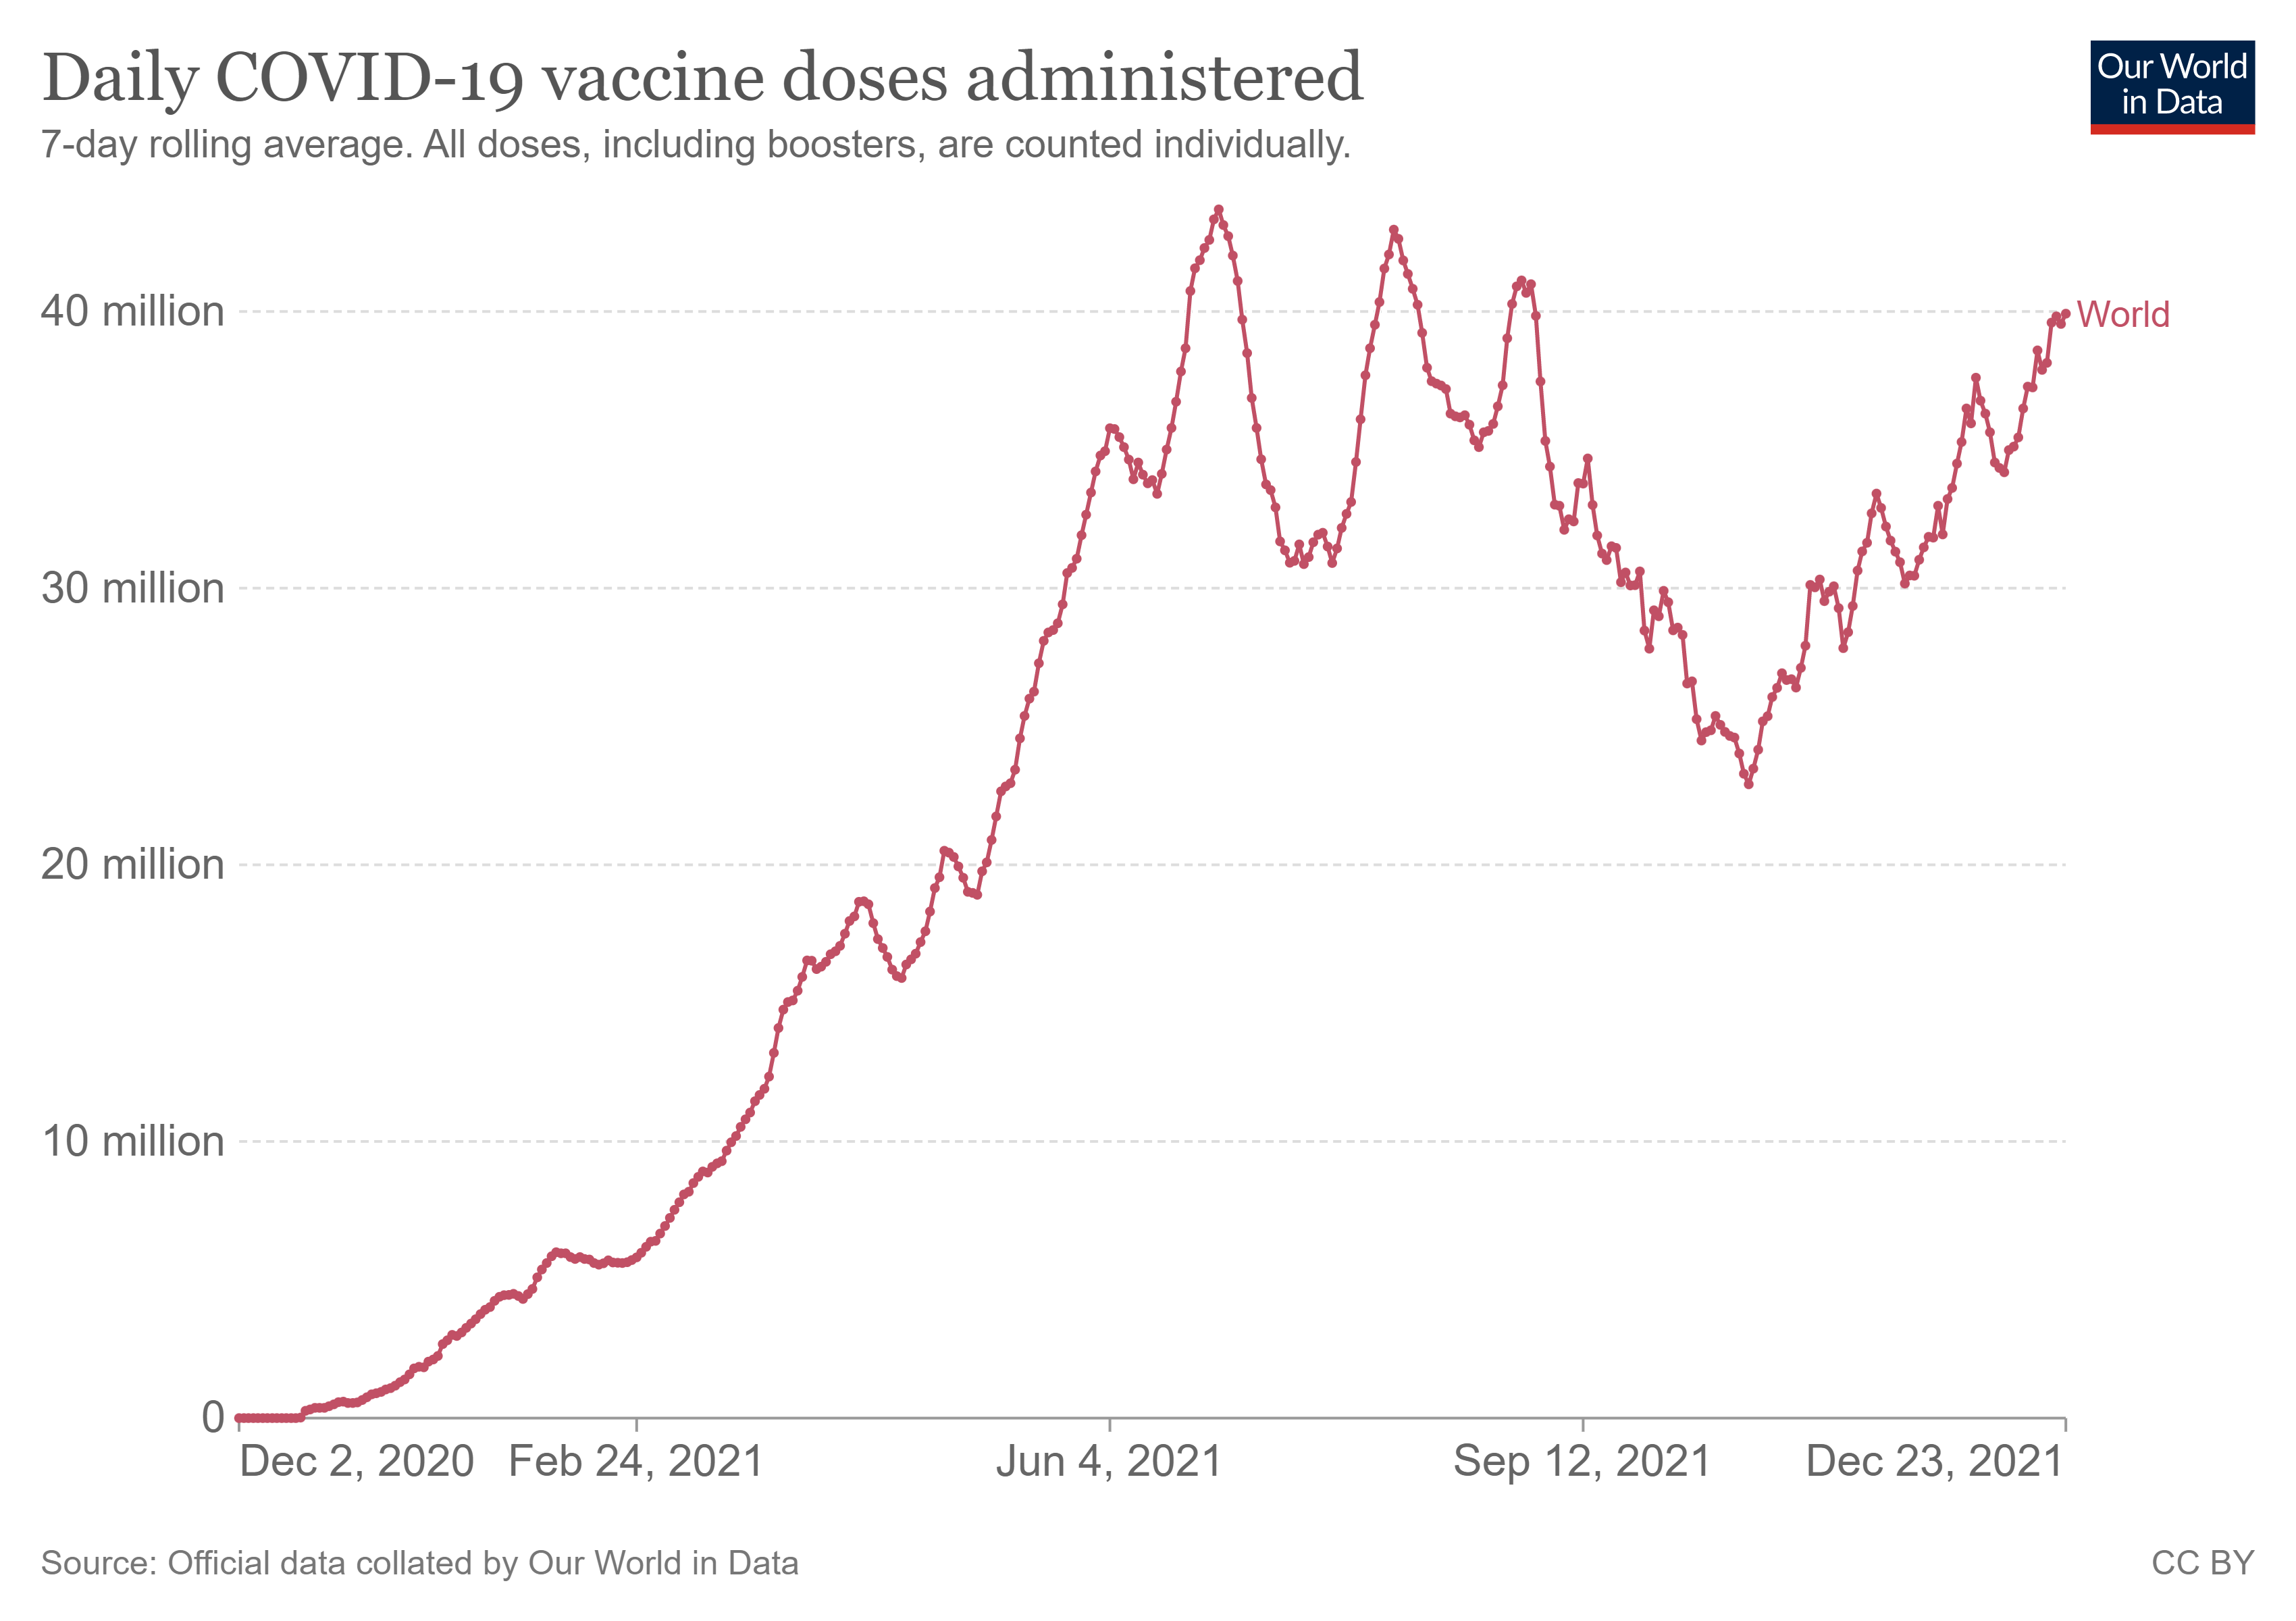
\includegraphics[width=15cm]{coronavirus-data-explorer.png}
\caption{World's Vaccination Rate in 2021}
\end{figure}

\subsubsection{How I acquired the data?}
I downloaded this dataset directly from Kaggle(https://www.kaggle.com/datasets/gpreda/all-covid19-vaccines-tweets). The dataset is in .csv format.

\subsubsection{Data Collection}
The data is collected from Twitter API using tweepy Python package. For each of the vaccine brands, the data provider used relevant search terms (most frequently used in Twitter to refer to the respective vaccine) to acquire data.

\subsubsection{The FAIRness of the data provider}
The dataset is following the FAIRness principle. The data was well-annotated with metadata and has a clear license. This is a public dataset on Kaggle, with CC0: Public Domain. I can easily access the dataset via Kaggle, without applying for permissions. There's no restriction. There are no certain types of analyses people cannot do with this dataset.

\subsubsection{Data Cleaning and Preprocessing}
Here are the data cleaning and preprocessing steps before analyzing the data.
\begin{itemize}
    \item Remove missing/duplicating data.\\
    Missing data and duplicated data are removed. After removing, there are 116054 rows remaining.
    \item Standardize the date column into 'yyyy-mm-dd' format.
    \item Remove URLs, hashtags, emojis, symbols, and punctuations in the text column, and change each row to lowercase. \\
    This is essential before tokenizing. Otherwise, it will cause trouble in future analyses.
    \item Tokenize the text column and remove stopwords.\\
    This step is needed for both building the model and analyzing the results.
    \item Get sentiment labels for all tweets using the classification model.\\
    Since the original data don't have labels, classification is needed to analyze the data. All tweets are labeled as -1(negative), 0(neutral), or 1(positive). The details about the model will be discussed in the next section.
\end{itemize}

\subsection{Exploratory Data Analysis}
After the data is labeled by the classification model, I did some exploratory data analysis. 

\begin{figure}[H]
\centering
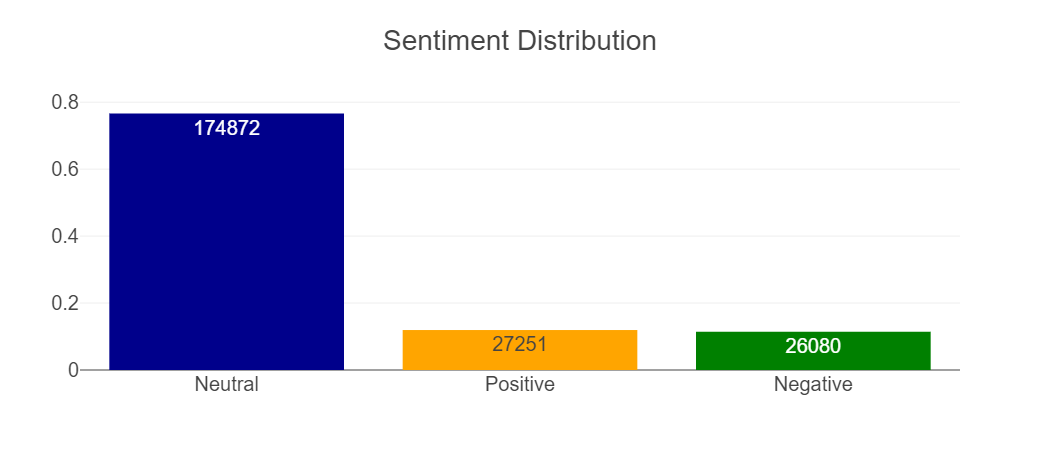
\includegraphics[width=15cm]{EDA1.png}
\caption{Sentiment Distribution after Labeling}
\end{figure}

About 75\% of the tweets are neutral. The positive tweets are slightly more than the negative tweets, while their proportions are about 12\%. 

Next, the overall sentiment of each vaccine brand is plotted. If the tweet in the text column contains one of the keywords ('Covaxin', 'Sinopharm', 'Sinovac', 'Moderna', 'Pfizer', 'BioNTech', 'Oxford', 'AstraZeneca', 'Sputnik') it will be counted towards the corresponding vaccine. One tweet might fall into multiple vaccine brands. After generating the subsets for each vaccine, an average sentiment score is calculated. The figure below shows the average sentiment score of each vaccine brand.

\begin{figure}[H]
\centering
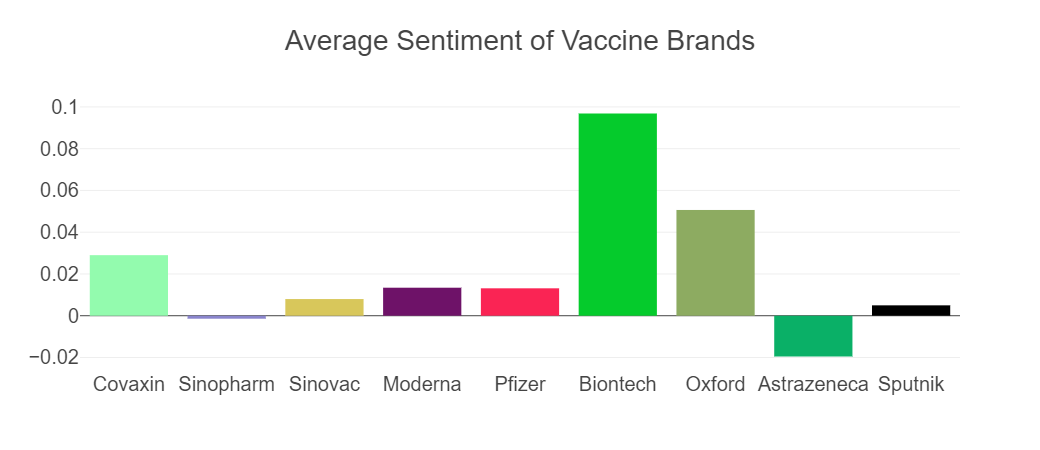
\includegraphics[width=15cm]{EDA2.png}
\caption{Average Sentiment of Vaccine Brands}
\end{figure}

From the above plot, BioNTech, Covaxin, and Oxford have the highest average sentiment score, while AstraZeneca has the lowest average sentiment score. AstraZeneca is the only vaccine with a negative score. It is interesting that the same vaccine with different names(Pfizer\&BioNTech, Oxford\&AstraZeneca) have different average scores. While BioNTech has a high positive sentiment score, Pfizer stays slightly above neutral. Oxford and AstraZeneca have polarized scores.

Similarly, the overall sentiment of each country is plotted. If the tweet in the user\_location column contains one of the keywords ('India', 'USA', 'Canada', 'Germany, 'Spain', 'Pakistan', 'UK', 'Brazil', 'Russia', 'Italy', 'Australia', 'France', 'Argentina', 'UAE', 'Israel', 'Mexico', 'Japan') it will be counted towards the corresponding country. One tweet will only be categorized into no more than one country. Here are two special cases: state abbreviations and city names are used to identify the USA, while "UK" and "England" are both used to identify the UK. After generating the subsets for each country, an average sentiment score is calculated. The figure below shows the average sentiment score of each country.

\begin{figure}[H]
\centering
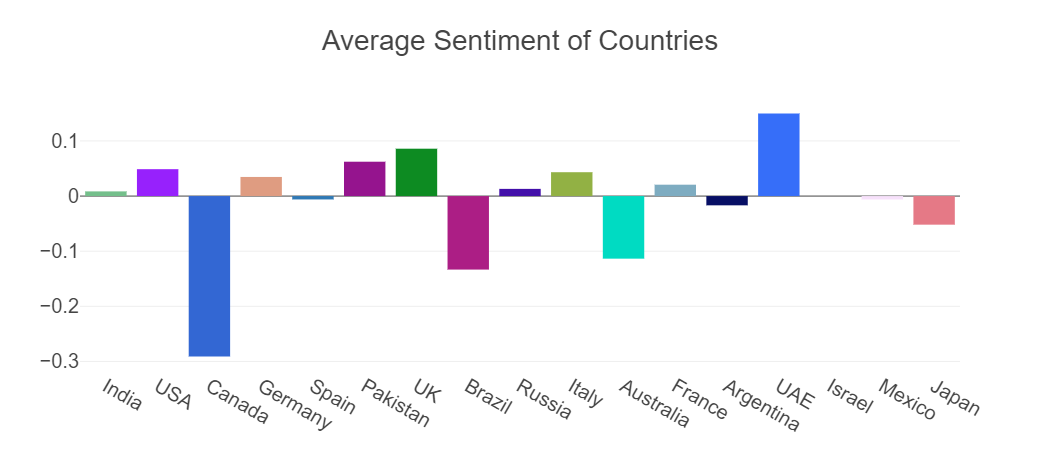
\includegraphics[width=15cm]{EDA3.png}
\caption{Average Sentiment of Countries}
\end{figure}

Most of the countries have a positive or negatively neutral overall result. UAE has the highest average sentiment score, and it is the only country with a score higher than 0.1. However, Canada, Brazil, and Australia have a nonnegligible low overall average sentiment score. It may be due to the negative attitude toward vaccination, or it may also be due to the lack of positive/neutral data.

Note that the results might be misleading since the sample size for each vaccine brand/country varies. Some low/high scores may be due to a lack of data. Also since Twitter is not the only social media platform for people to leave feedback, the results cannot represent the overall reputation of a specific vaccine in a specific country.

\section{Model}

\subsection{Basic Information}
\subsubsection{Training and Validation Data}
Since the vaccine tweets dataset is not labeled, I used another dataset to train and validate my model. This dataset is called Complete Tweet Sentiment Extraction Data. I downloaded the dataset directly from Kaggle(https://www.kaggle.com/datasets/maxjon/complete-tweet-sentiment-extraction-data). The dataset is in .csv format and follows the FAIRness principle. The training set contains 90\% of the data, while the validation set holds the rest 10\%.

\subsubsection{Data Cleaning and Preprocessing}
This dataset has several columns, however, I only need the "text" column and the "new\_sentiment" column to train the model.

text: Contains 31329 raw tweets.

new\_sentiment: Contains the corresponding sentiment labels for 31329 tweets.

The data cleaning and preprocessing procedures are exactly the same as the procedures for the vaccine tweets dataset.  Please refer to the data cleaning subsection in the previous section for more information.

\subsubsection{Training and Fine-tuning}
After data cleaning and preprocessing, it's time to train the model. I started with a pre-trained model called BERT. BERT stands for “Bidirectional Encoder Representation with Transformers”, and it is a pre-trained language model. To put it in simple words, BERT extracts patterns or representations from the data or word embeddings by passing them through an encoder. BERT falls into a self-supervised model. That means, it can generate inputs and labels from the raw corpus without being explicitly programmed by humans. I think BERT is a good fit for predicting sentiments.

My model is built from the BERT model using PyTorch. I adjusted the model parameters and fine-tuned them with the training and validation dataset. 

\subsection{Model Performance}
The model has a 75\% training Accuracy, with a training loss of 0.59. As for the validation accuracy, it reaches 80\% with a validation loss of 0.48.

\begin{figure}[H]
\centering
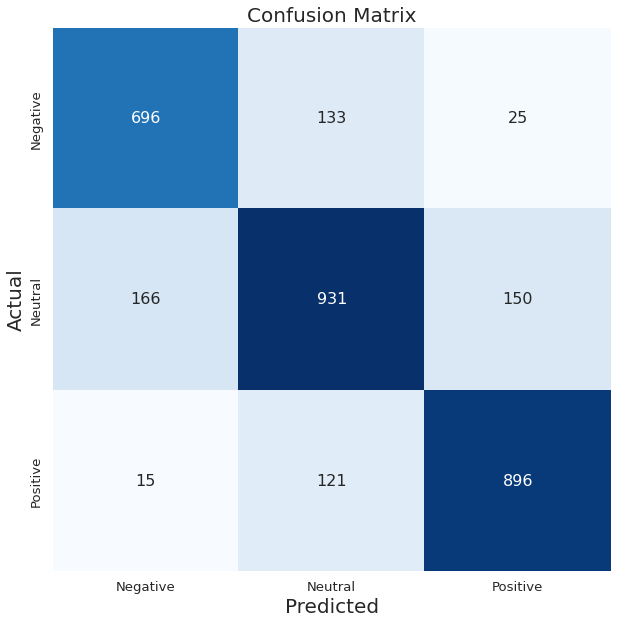
\includegraphics[width=10cm]{confusion_matrix.png}
\caption{Confusion Matrix on the Validation Dataset}
\end{figure}

By checking the confusion matrix, I can tell the model can clearly distinguish between positive and negative tweets with very few errors in the bottom left corner and the upper right corner. However, it makes mistakes when distinguishing between negative and neutral, or positive and neutral. This is acceptable since if you check the probability breakdown, the probability for negative\&neutral or positive\&neutral are very close, and by the nature, the model chose to label the text with the sentiment whose probability is the highest. Also, there are some cases hard to label even for humans. I think the model performance is overall acceptable and can be used to label the COVID-19 vaccine tweets dataset.

\section{Data Analysis, Results and Interesting Findings}

With the data visualization methods, I analyzed and investigated the dataset, summarized its main characteristics, and compared the changes over time for different categories. I've conducted two analyses, to answer the corresponding research question.

\subsection{Word Cloud Analysis}

\subsubsection{Research Questions}
What are the most common words in tweets with different sentiment?

What are the most common words in tweets about different vaccine brands?

What are the most common words in tweets in different countries?

\subsubsection{Results and Interesting Findings}

I have implemented three interactive word clouds in my Web application. The user can choose from different sentiments, countries, and vaccine brands to generate different word clouds for the top 50 most common words. Word frequencies and percentages of the total are available if the user moves their mouse to the corresponding word. The larger the word is, the higher its frequency is among all qualifying tweets.

\begin{enumerate}

    \begin{figure}[H]
    \centering
    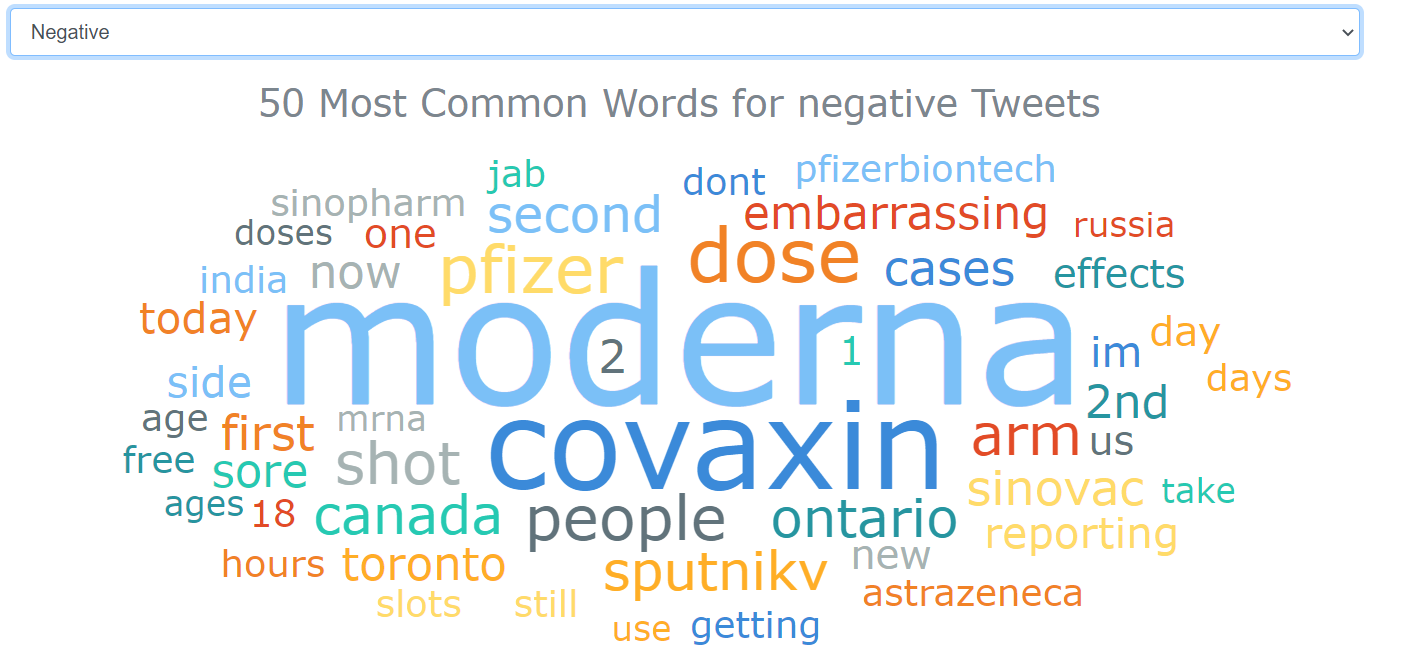
\includegraphics[width=10cm]{Negative.png}
    \caption{Word Clouds for Tweets in Japan}
    \end{figure}
    \item "Canada", "Ontario" and "Toronto" appeared on the word cloud for negative tweets. This matched the EDA result that tweets in Canada have the lowest average sentiment score.
    \item It seems that all brands of vaccines have positive feedback. "good" and "effective" appeared on all word clouds for different vaccine brands.
    \item It's interesting to point out the Japan is the only country whose word cloud has nothing to do with itself. Everything shown on Japan's word cloud is relevant to the US (e.g. US politicians' names).
    \begin{figure}[H]
    \centering
    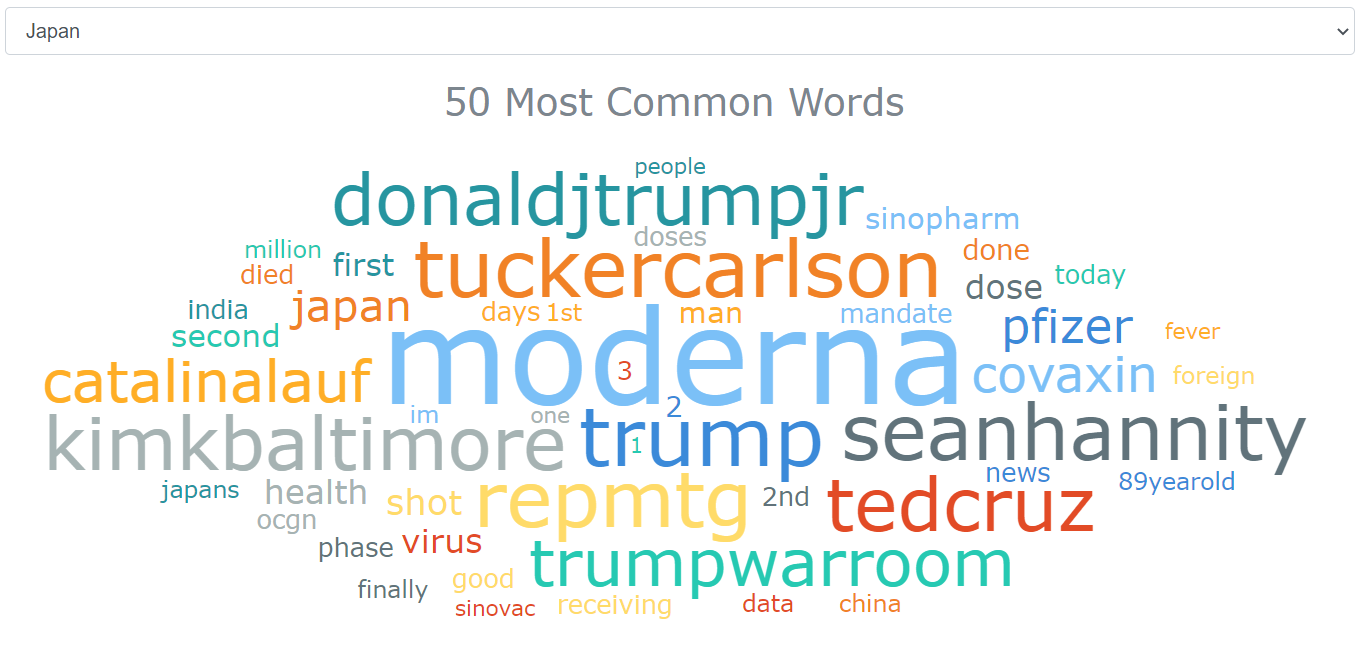
\includegraphics[width=10cm]{Japan.png}
    \caption{Word Clouds for Tweets in Japan}
    \end{figure}
    \item The main topics in the COVID-19 vaccines tweets are availabilities, effectiveness, number of doses, policies, and side effects. Different vaccine brands are also discussed frequently. 
\end{enumerate}

\subsection{Timeseries Analysis}

\subsubsection{Research Questions}

How does the sentiment change over time?

Do they have a common trend?

\subsubsection{Results and Interesting Findings}

I have implemented three interactive time series plots in my Web application. The user can either plot the average sentiment over time for different vaccines and different countries, or plot the number of tweets over time in a selected sentiment. Average sentiment scores and tweet counts are available if the user moves their mouse to the corresponding date. 

\begin{enumerate}
    \item As a common trend for Pfizer/BioNTech and Moderna, we can see that in the initial stages the sentiment seems to be above neutral. However, when it comes to the end of the year, the overall sentiment tends to move negatively.
    \item As for all other vaccines, the overall sentiment stays neutral. However, this may be due to the lack of data.
    \item The countries with an appropriate data size are UK, US, and Canada. They have a common trend where the overall sentiment score moves from the positive side to the negative over time. Canada's scores are on the negative side all the year. As for other countries, the data size is not enough thus useful results cannot be generated from the plots.
    \item The discussion of COVID-19 vaccines on Twitter kept increasing and reached its peak in the middle of 2021, then decreases till the end of the year. When CDC releases new changes in vaccination policies, people are more likely to discuss more on Twitter. Neutral is the dominant sentiment, but it could be argued that Positive & Negative sentiments were fairly equal.
\end{enumerate}

\section{Server API and the Web Front-end}

The local Web application is built with Python flask, along with some HTML and CSS, and some Javascript/JQuery. There are 7 app routes and 7 APIs.

\subsection{API}
The APIs are used to generate data for interactive plots, or to generate classification output using the model. All outputs are in JSON format.

\begin{itemize}
    \item @app.route('/wordcloud\_api/\textless string:vax\_name\textgreater'): Returns JSON-encoded data generating a word cloud given a vaccine brand.
    \item @app.route('/wordcloud\_api/senti/\textless string:senti\textgreater'): Returns JSON-encoded data generating a word cloud given a sentiment.
    \item @app.route('/wordcloud\_api/country/\textless string:country\textgreater'): Returns JSON-encoded data generating a word cloud given a country name.
    \item @app.route('/timeseries\_api/varianceVStime/\textless string:vax\_name\textgreater'): Returns JSON-encoded data generating a timeseries graph given a vaccine brand.
    \item @app.route('/timeseries\_api/varianceVStime\_Country/\textless string:country\textgreater'): Returns JSON-encoded data generating a timeseries graph given a country name.
    \item @app.route('/timeseries\_api/SDT/\textless string:senti\textgreater'): Returns JSON-encoded data generating a bar graph given a sentiment.
    \item @app.route('/model\_api/\textless string:user\_text\textgreater'): Returns JSON-encoded data generating the predicted results from the model given a user input.
\end{itemize}

\subsection{Web Front-end}
There are 7 total pages.

\begin{itemize}
    \item @app.route('/'): Home Page. Displays the structure of the Web application.
    \item @app.route('/data'): Data Page. Displays everything about the dataset.
    
    \begin{figure}[H]
    \centering
    \begin{minipage}[H]{.5\textwidth}
      \centering
      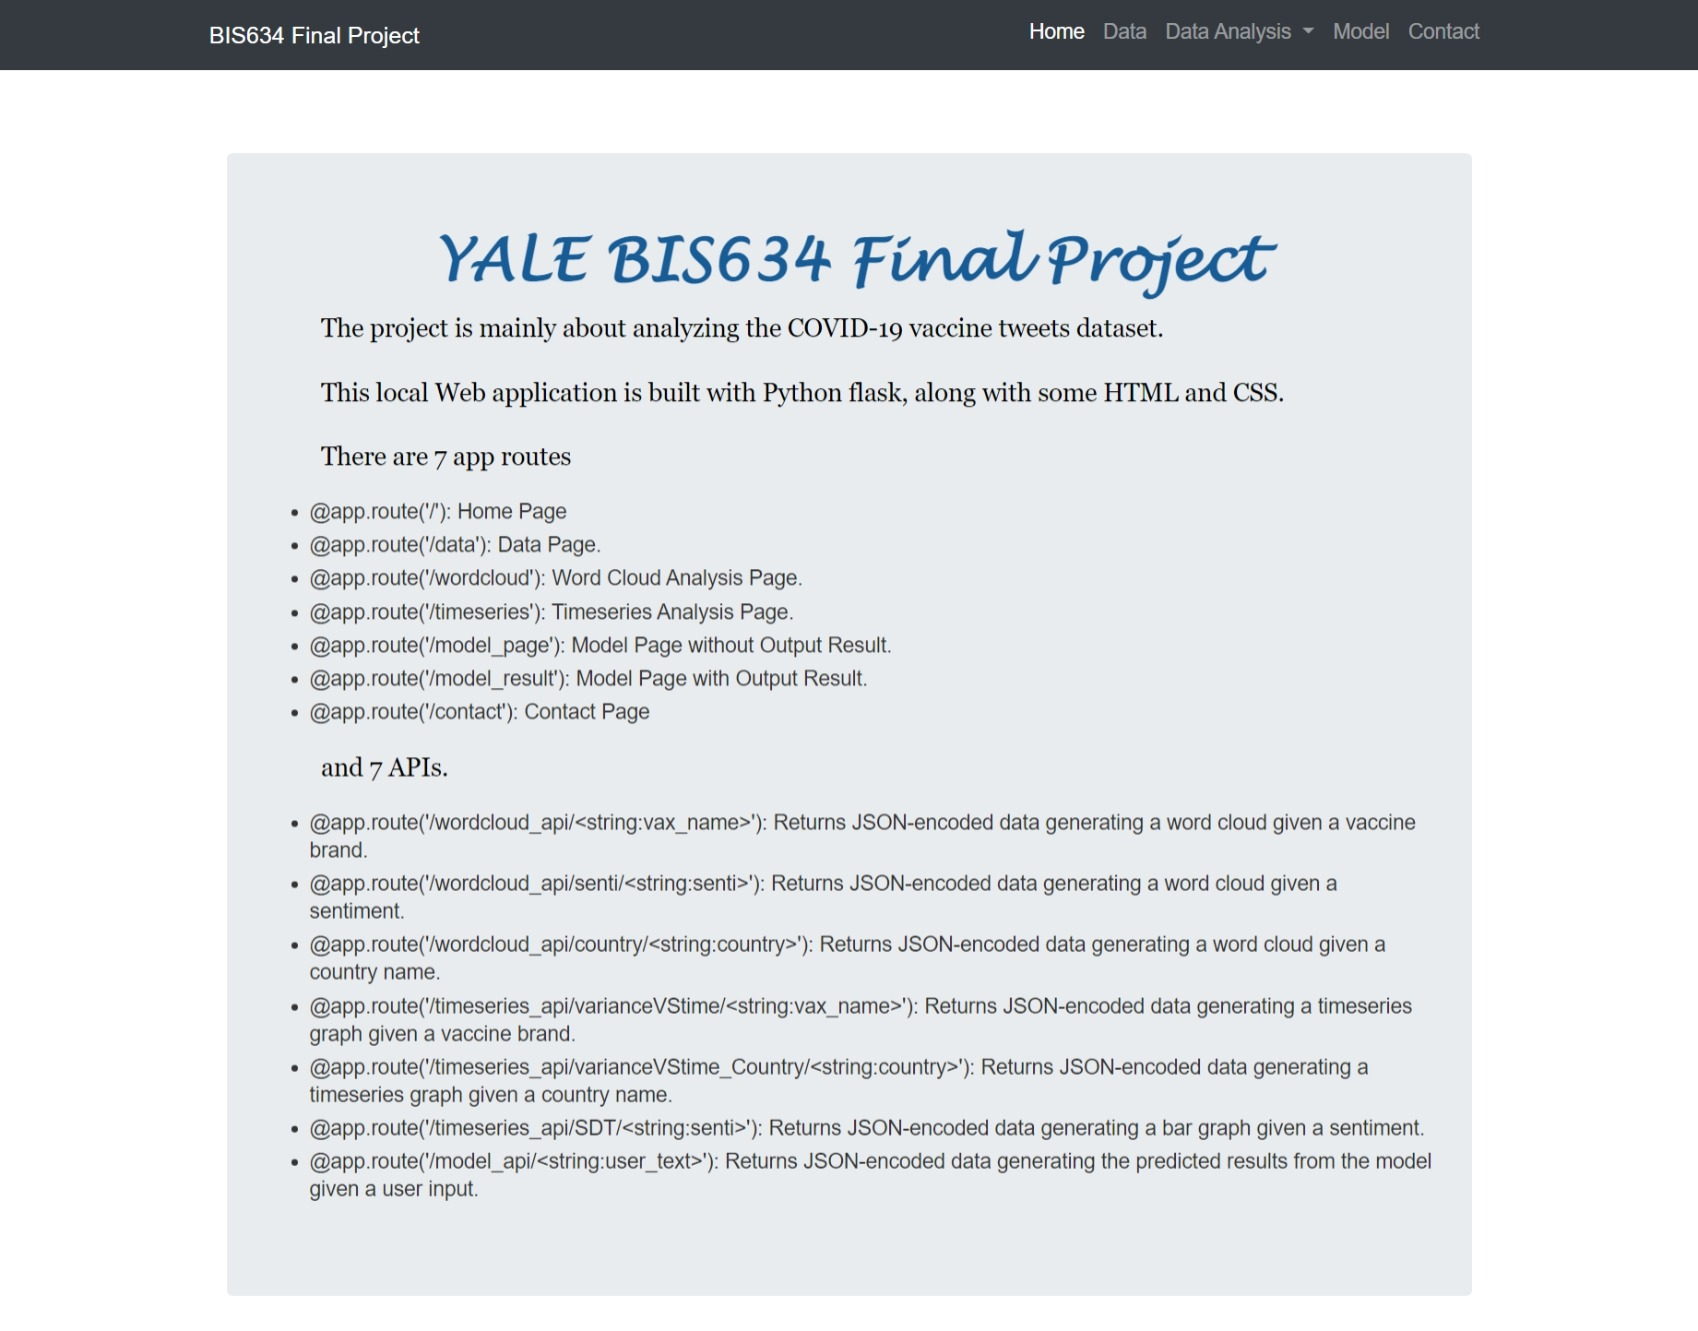
\includegraphics[width=\linewidth]{HomePage.jpeg}
      \caption{Home Page}
    \end{minipage}%
    \begin{minipage}[H]{.5\textwidth}
      \centering
      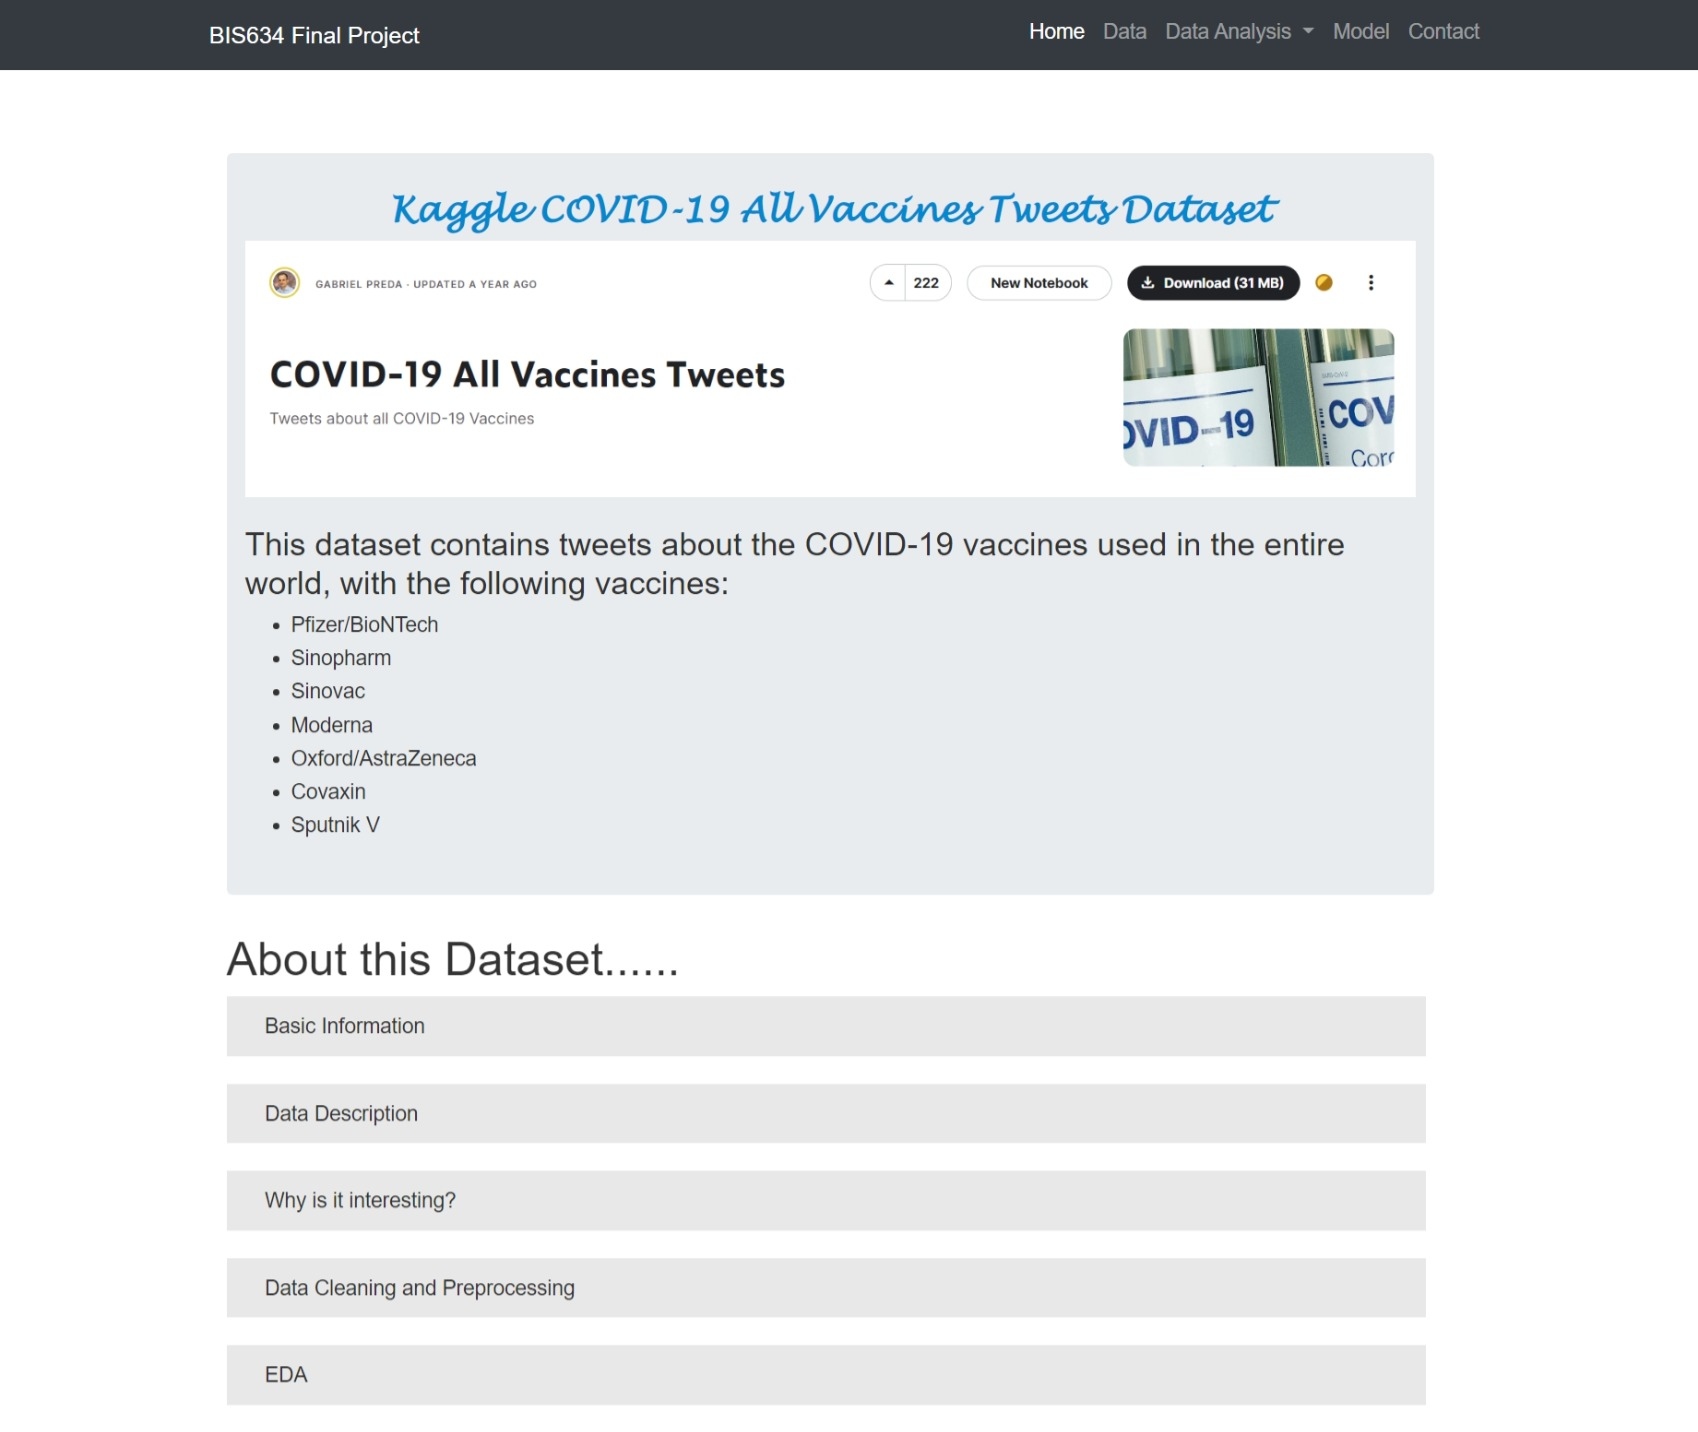
\includegraphics[width=\linewidth]{DataPage.jpeg}
      \caption{Data Page}
    \end{minipage}
    \end{figure}
    
    \item @app.route('/wordcloud'): Word Cloud Analysis Page. Displays the interactive word clouds and the findings.
    \item @app.route('/timeseries'): Timeseries Analysis Page. Displays the interactive timeseries plots and the findings.
    \begin{figure}[H]
    \centering
    \begin{minipage}[H]{.5\textwidth}
      \centering
      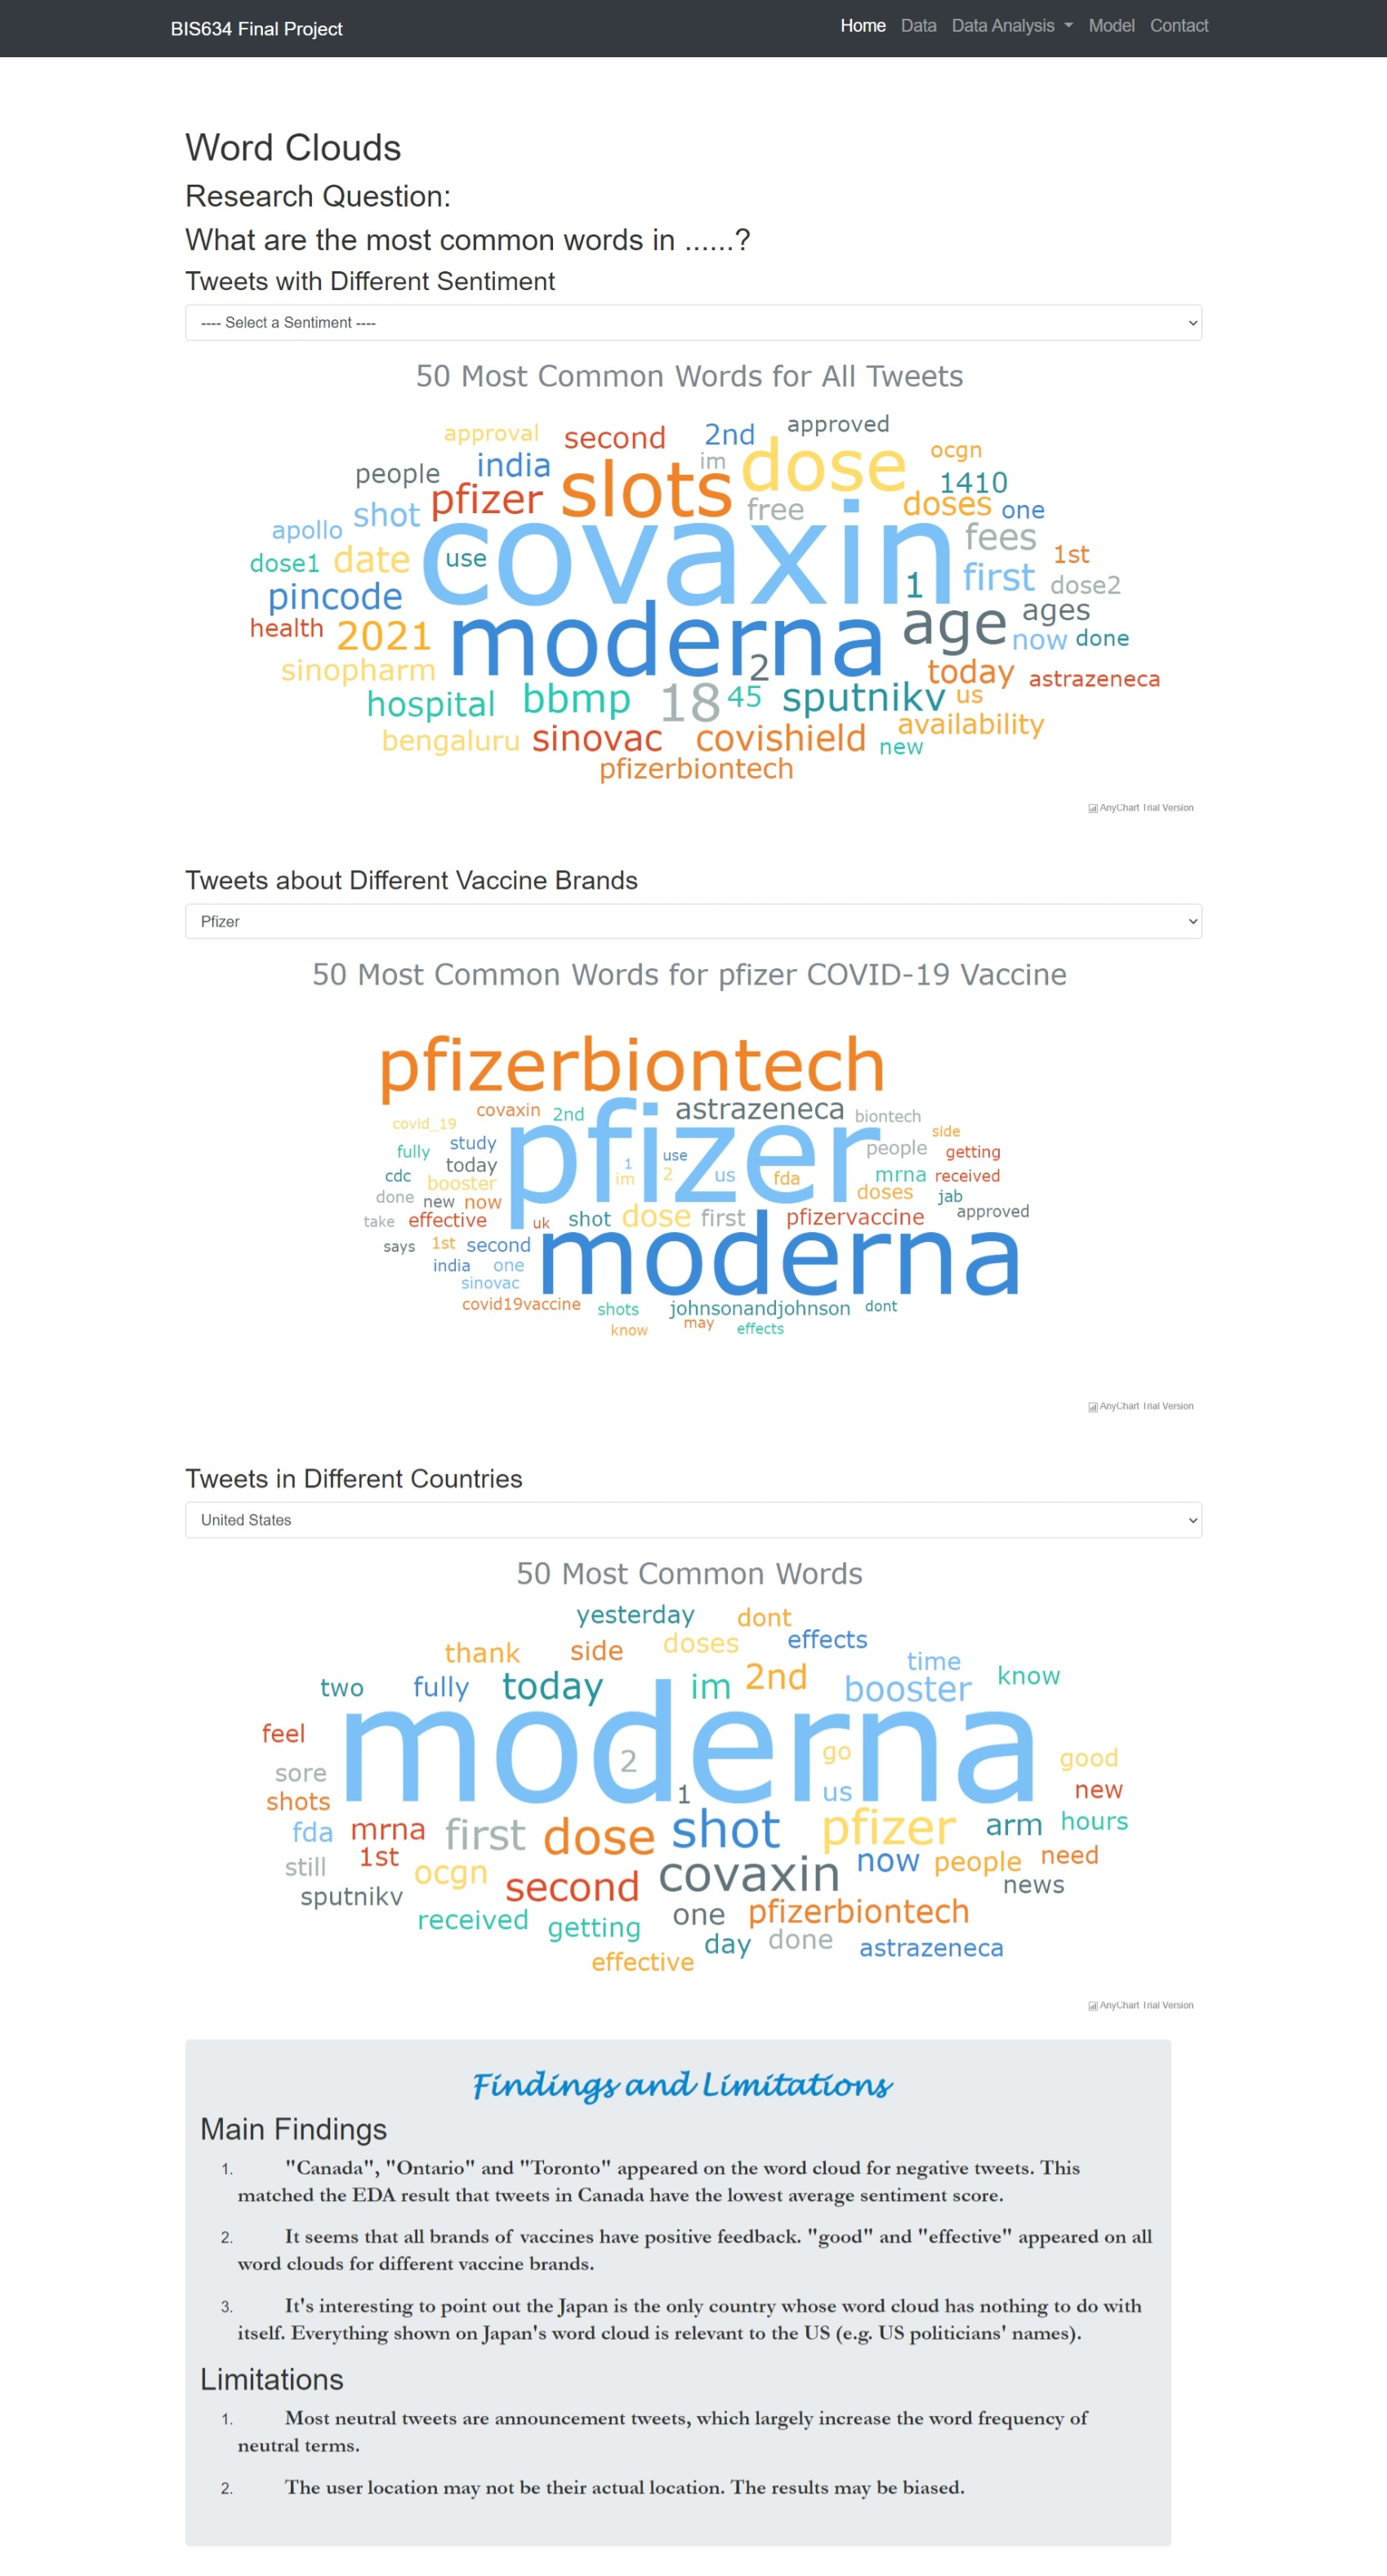
\includegraphics[width=\linewidth]{WordCloud.jpeg}
      \caption{Word Cloud Analysis Page}
    \end{minipage}%
    \begin{minipage}[H]{.5\textwidth}
      \centering
      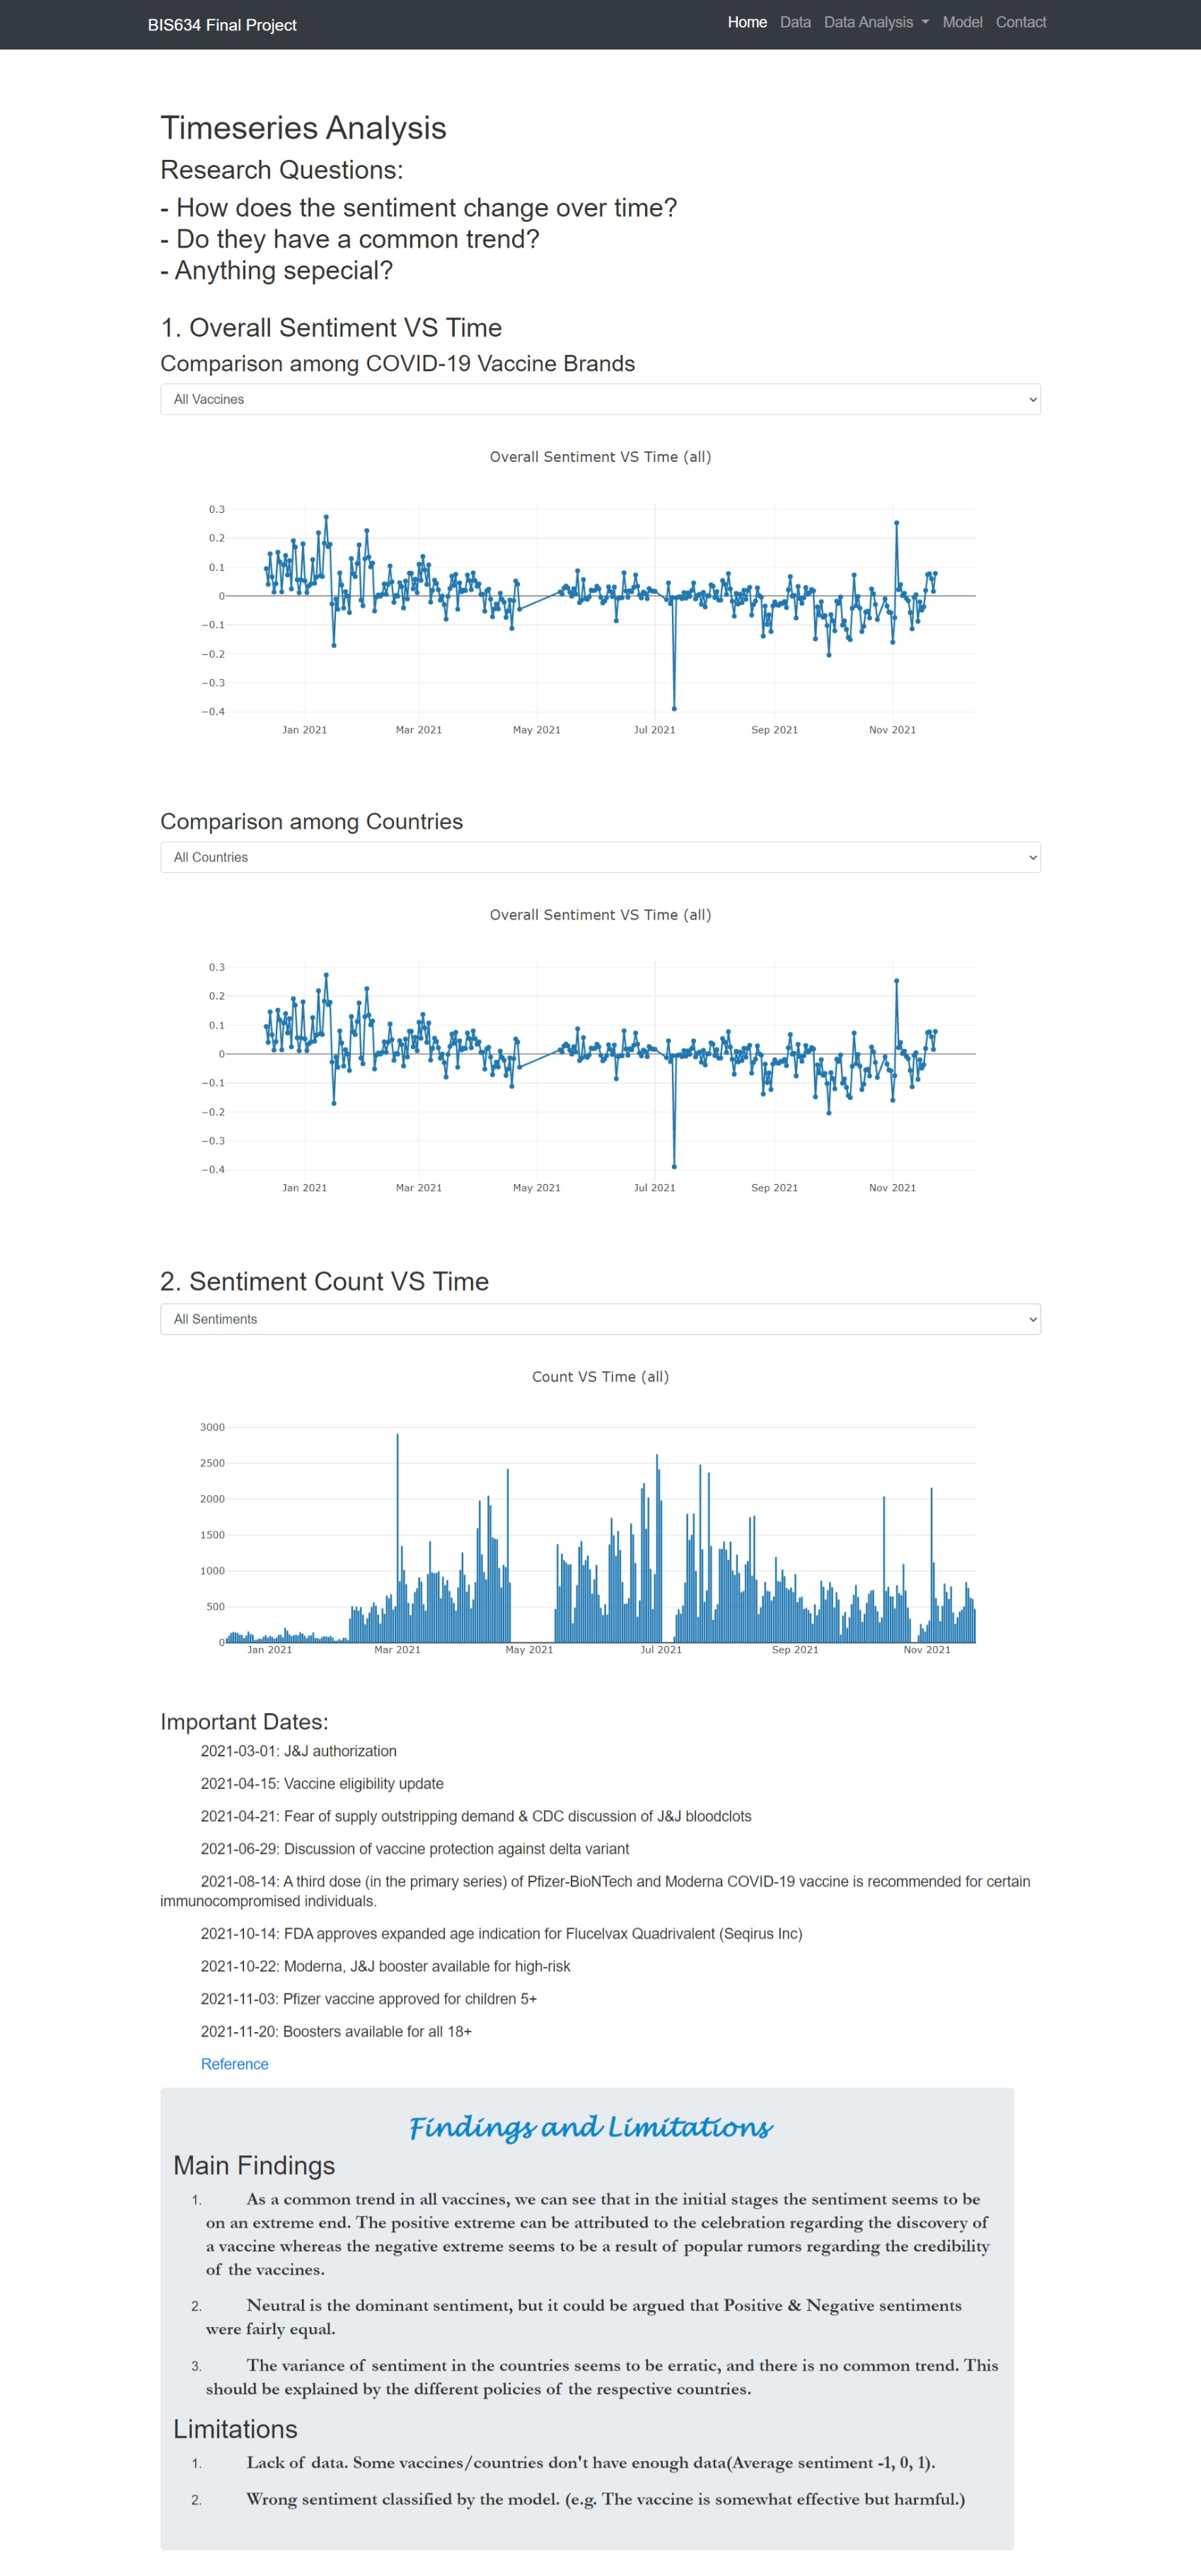
\includegraphics[width=\linewidth]{Timeseries.jpeg}
      \caption{Timeseries Analysis Page}
    \end{minipage}
    \end{figure}
    \item @app.route('/model\_page'): Model Page without Output Result. Displays the input box and the model information.
    \item @app.route('/model\_result'): Model Page with Output Result. Displays the input box, model output, and the model information.
    \item @app.route('/contact'): Contact Page. Displays my contact information and Web application source code.
    \begin{figure}[H]
    \centering
    \begin{minipage}[H]{.5\textwidth}
      \centering
      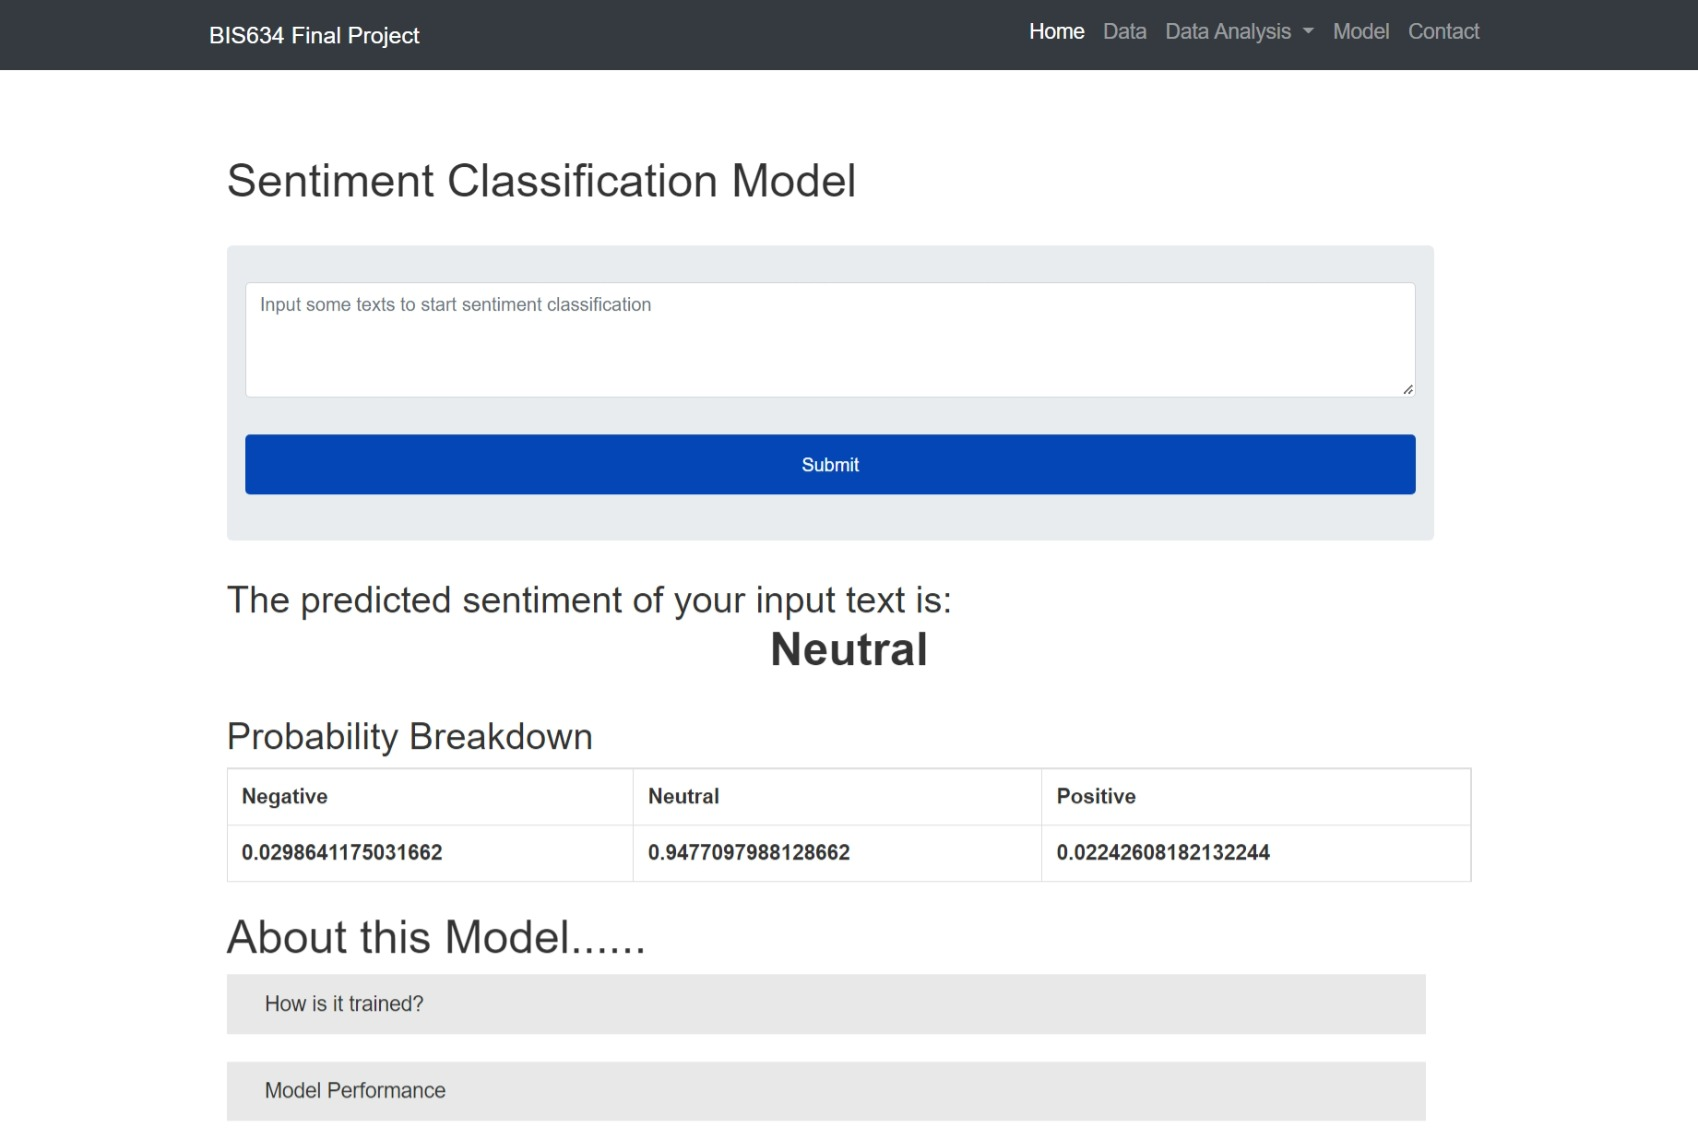
\includegraphics[width=\linewidth]{ModelPageWithInput.jpeg}
      \caption{Model Page/Result Page}
      \label{fig:sub1}
    \end{minipage}%
    \begin{minipage}[H]{.5\textwidth}
      \centering
      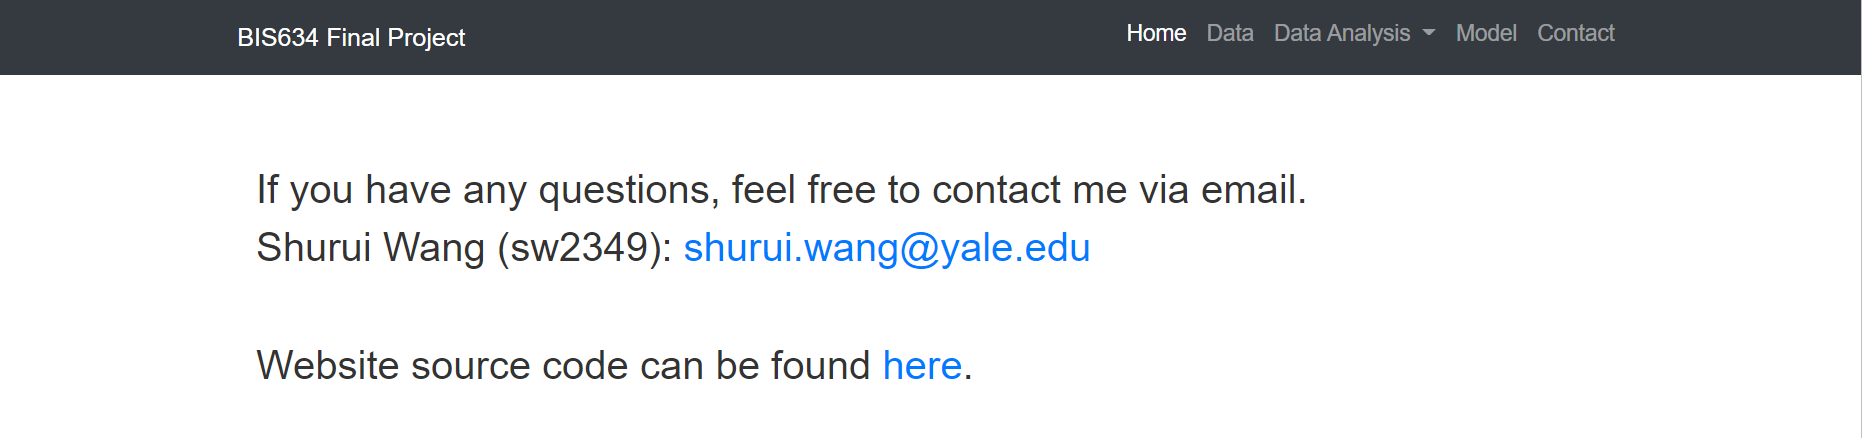
\includegraphics[width=\linewidth]{ContactPage.png}
      \caption{Contact Page}
      \label{fig:sub2}
    \end{minipage}
    \end{figure}
\end{itemize}

\section{Limitations}
\begin{enumerate}
\item Due to the lack of data, some countries/vaccines have a relatively low sample size which leads to an unusually high/low average sentiment score.  Thus, the results may be misleading and inconclusive.
\item Since the sentiment labels are predicted using the model, and the model accuracy is about 80\%, it is possible that the labels are wrongly marked for some tweets. For example, some neutral tweets are not necessarily neutral. This may lead to analysis bias.
\item Since Twitter is not the only social media platform for people to leave feedback, the results cannot represent the overall reputation of a specific vaccine in a specific country. Also, since the data is outdated, the analysis results only represent 2021, not now.
\end{enumerate}

\section{Unexpected Difficulties}
\begin{enumerate}
\item Since I'm not familiar with JavaScript and JQuery, it is extremely hard for me to make the interactive plots work on my Website. I have no idea how to get the user input/selected values from dropdown menus and implement them on my website. Also, the tutorials online match my needs are limited. 
\item Another difficulty is the unexpectedly long time to train the machine learning model and predict the results. A minor mistake in data cleaning will lead to re-running all the code which was a painful and time-consuming experience. 
\end{enumerate}
Finally, I overcome all difficulties and made everything work.

\section{Appendix}

Here are links to my data sources:

1. COVID-19 All Vaccines Tweets Dataset. 

https://www.kaggle.com/datasets/gpreda/all-covid19-vaccines-tweets

2. Complete Tweet Sentiment Extraction Data.

https://www.kaggle.com/datasets/maxjon/complete-tweet-sentiment-extraction-data

\end{document}